\documentclass[laboratorio]{guia}

\def \practnum {11}
\def \practica {Redes de difracci\'on}

\def \materia {Laboratorio de F\'\i sica II para Qu\'\i micos}
\def \periodo {2do. Cuatrimestre de 2015}
\def \catedra {Pablo Cobelli}
\def \website {http://materias.df.uba.ar/f2qa2015c2}

\usepackage{graphics}
\usepackage{amsmath}
\usepackage{amsfonts}
\usepackage{graphicx}
\usepackage{float}
\usepackage{wrapfig}
\usepackage{subfigure}
\usepackage{bm}
\usepackage{grffile}
\usepackage{color}
\usepackage{framed}
\usepackage[utf8]{inputenc}
\usepackage[T1]{fontenc}
\usepackage{lmodern}
\usepackage{circuitikz}
\usepackage[spanish]{babel}
\usepackage{babelbib}
\selectbiblanguage{spanish}



%----------------------------------------------------------
% Agrega al path de figuras el subdirectorio con el mismo
%     nombre que el archivo principal del proyecto
\graphicspath{{./\jobname/}}

%----------------------------------------------------------
% Definicion del entorno 'sabermas'
\makeatletter
\definecolor{shadecolor}{rgb}{0.89,0.91,0.94}
\newenvironment{sabermas}[1]{%
\vfill
\begin{shaded}
  \begin{center}
  {\textsection{Para saber m\'as}}
  \end{center}
  #1
\sf } 
{%
\end{shaded}%
}
\makeatother

%----------------------------------------------------------
% Definicion del entorno 'problema'
\newcounter{ContadorProblema}
\setcounter{ContadorProblema}{0}
\newcounter{TieneFiguraAsociada}
\setcounter{TieneFiguraAsociada}{0}
\newcounter{UbicacionFigura}
\setcounter{UbicacionFigura}{0}

\newenvironment{problema}[2][]
{%
    \ifx\relax#1\relax%
        \setcounter{TieneFiguraAsociada}{0}
        \else
        \setcounter{TieneFiguraAsociada}{1}
    \fi
    \def \archivofigura {#1}
    % 
    \refstepcounter{ContadorProblema}
    \noindent%
    \ifnum\value{TieneFiguraAsociada} < 1%
        {\sffamily \bfseries Problema \arabic{ContadorProblema}.}
        %{\sc {#1}}%
        \par\nobreak\par\nobreak%
        \medskip 
    \else
        % Va con figura; resta determinar de que lado.
        \ifnum\value{UbicacionFigura} < 1
            % Poner la figura del lado derecho
            \begin{minipage}{12.25cm}
            {\sffamily \bfseries Problema \arabic{ContadorProblema}.}
            %{\sc {#1}}%
            \par\nobreak\par\nobreak%
            \medskip 
        \else
            % Poner la figura del lado izquierdo
            \begin{minipage}{4.5cm}
                \centering
                \includegraphics[width=4.5cm]{\archivofigura}
                {\footnotesize {\sffamily Esquema asociado al 
                problema \arabic{ContadorProblema}}.}
            \end{minipage}\hfill%
            \begin{minipage}{12.25cm}
                {\sffamily \bfseries Problema \arabic{ContadorProblema}.}
                %{\sc {#1}}%
                \par\nobreak\par\nobreak%
                \medskip 
        \fi
    \fi
}
{%
    \ifnum\value{TieneFiguraAsociada} < 1%
        % \par \bigskip \vskip 0.3cm
    \else
        % Va con figura; resta determinar de que lado.
        \ifnum\value{UbicacionFigura} < 1
            % Poner la figura del lado derecho
            \end{minipage}\hfill%
            \begin{minipage}{4.5cm}
                \centering
                \includegraphics[width=4.5cm]{\archivofigura}
                {\footnotesize {\sffamily Esquema asociado al 
                problema \arabic{ContadorProblema}}.}
            \end{minipage}
        \else
            % Poner la figura del lado izquierdo
            \end{minipage}%
        \fi
    \fi
    \setcounter{TieneFiguraAsociada}{0}
    \par \bigskip \vskip 0.3cm
    % Permutamos el valor de la ubicacion
    \ifnum\value{UbicacionFigura} < 1
        \setcounter{UbicacionFigura}{1}
    \else
        \setcounter{UbicacionFigura}{0}
    \fi
}

%----------------------------------------------------------
% Definicion/Redefinicion de estilos
\renewcommand{\vec}[1]{\ensuremath{\mathbf{#1}}}



\hyphenation{ coe-fi-cien-tes coe-fi-cien-te au-to-va-lor
              au-to-va-lo-res co-rres-pon-der pro-ble-ma 
              cual-quie-ra po-la-ri-za-cio-nes }

\graphicspath{{./redes/}}

\begin{document}
\objetivo{Medir el espectro de emisi\'on de una l\'ampara de sodio (Na) 
    empleando redes de difracci\'on. Determinar los l\'\i mites del espectro 
    visible utilizando una fuente de luz blanca. 
\tematicas{Redes de difracci\'on por reflexi\'on y transmisi\'on, espectro de
emisi\'on. }}
\maketitle

\section{Redes de difracci\'on}

Una red de difracci\'on es una estructura repetitiva que se utiliza para
introducir una perturbaci\'on peri\'odica en un frente de onda. Entre las
configuraciones m\'as sencillas se encuentra la red plana de transmisi\'on;
formada por una serie de rendijas id\'enticas y equiespaciadas. 

Si un frente de ondas plano incide sobre una red, el patr\'on de difracci\'on
observado sobre una pantalla alejada (difracci\'on de Fraunhoffer) presenta
una distribuci\'on de intensidad dada por

\begin{equation}
    I(\theta) = I_0 \: \left( \frac{\sin \beta}{\beta} \right)^2 \: 
    \left[ \frac{\sin N\alpha}{\sin \alpha}\right]^2,
    \label{eq:difraccion}
\end{equation}
donde 
\begin{align*}
    \alpha &= \frac{\pi b}{\lambda} \: 
    \left(\sin \theta - \sin \theta_0 \right), \\
    \beta  &= \frac{\pi a}{\lambda} \: 
    \left(\sin \theta - \sin \theta_0 \right), \\
\end{align*}
siendo $a$ el ancho de cada rendija de la red, $b$ el espaciado entre ellas,
$\lambda$ la longitud de onda del haz incidente, 
$\theta_0$ el \'angulo que forma el haz incidente con la red y $\theta$ la
posici\'on angular del haz cuya intensidad estamos observando en la pantalla.

En la ecuaci\'on~\eqref{eq:difraccion}, el factor entre par\'entesis 
est\'a asociado a la {\it difracci\'on} producida por cada rendija
presente en la red. El factor entre corchetes, por otro lado, da cuenta de la 
{\it interferencia} entre las $N$ rendijas de la red. 

Para valores espec\'\i ficos de $\alpha$ y $\beta$, la intensidad registrada
$I(\theta)$ presentar\'a m\'aximos principales sobre la pantalla de 
observaci\'on, entre los cuales observar\'a tambi\'en m\'aximos secundarios.
El resultado de esta combinaci\'on es la interferencia {\it modulada} por
la figura de difracci\'on. Dado que en este caso la campana central de 
difracci\'on resulta mucho m\'as ancha que la separaci\'on entre los m\'aximos
de interferencia, los \'ordenes que usualmente se observan con una red 
corresponden a la interferencia producida por las $N$ rendijas que componen
la red de difracci\'on. Si nos concentramos entonces en el factor de 
interferencia, encontramos que la intensidad resulta m\'axima cuando se
verifica

\begin{equation}
    \alpha = m \pi, \quad \quad \text{siendo } m = 0, \pm 1, \pm 2, \ldots.
\end{equation}

En base a esta condici\'on, el entero $m$ recibe el nombre de {\it orden de
interferencia}. Reemplazando este valor en la expresi\'on para $\alpha$, 
surge la condici\'on

\begin{equation}
    \sin \theta_m - \sin \theta_0 = m \frac{\lambda}{b},
\end{equation}
a partir de la cual es posible determinar el \'angulo $\theta_m$ 
correspondiente al m\'aximo de interferencia de orden $m$. Esta expresi\'on
se denomina com\'unmente {\it ecuaci\'on de la red}. 

Observe que si el haz incidente no es monocrom\'atico, la ecuaci\'on de la
red sigue teniendo validez, pero constituye ahora una condici\'on que se
cumple para cada longitud de onda considerada. Reflexione acerca de c\'omo es
la relaci\'on entre la posici\'on angular del m\'aximo de interferencia y la
longitud de onda de la luz considerada. A mayor longitud de onda, ?`la 
desviaci\'on del haz es mayor o menor?

Analice c\'omo es la distribuci\'on de los m\'aximos cuando la incidencia 
es normal ($\theta_0 = 0$) y cuando no lo es ($\theta_0 \neq 0$).
Verifique su análisis comparando con la figura \ref{fig:ordenes} 

\begin{figure}
  \centering
  \def\svgwidth{\columnwidth}
  \input{./redes/ordenes.pdf_tex}
  \caption{Numeración de órdenes de los máximos ante incidencia no normal.}
  \label{fig:ordenes}
\end{figure}



\section{Medici\'on del espectro de emisi\'on de una l\'ampara de sodio}

En esta pr\'actica se medir\'an la(s) longitud(es) de onda emitida(s) por una
l\'ampara de sodio (Na) utilizando para ello una red de transmisi\'on y un 
goni\'ometro (instrumento que se utiliza para medir \'angulos).

Los pasos importantes a seguir en esta experiencia son:

\begin{enumerate}
\item {\bf Calibraci\'on del goni\'ometro}. 

El goni\'ometro consta de una platina giratoria solidaria a un limbo graduado,
sobre la cual se coloca la red. Un colimador, para crear un haz incidente de 
rayos paralelos, y un anteojo que permite llevar el plano de observación al 
infinito, el anteojo es móvil y posee un vernier para medir el ángulo de giro
sobre el limbo graduado. El anteojo tiene un retículo en forma de cruz que 
permite definir mejor las posiciones que se miden.

Antes de medir, el dispositivo debe ser ajustado para trabajar bajo las 
condiciones de difracción de Fraunhofer e incidencia normal. Para ello debe 
enfocar el colimador y el anteojo. Primero se enfoca el anteojo mirando un 
objeto distante (enfoque a infinito) desplazando el ocular del tubo. Luego se 
enfoca el colimador enfrentándolo al anteojo y desplazando la rendija que se 
halla adherida a él hasta obtener una imagen nítida de ella.

A continuación se debe ubicar la red paralela al eje del goniómetro y 
aproximadamente perpendicular al haz colimado. La red se encuentra paralela 
al eje cuando la imagen de la rendija a través de la red se halle centrada 
y paralela al eje vertical del retículo. Para lograr posicionarla 
u correctamente la platina cuenta con tres tornillos de nivelación.


\item {\bf Posicionamiento de la red en el goni\'ometro.} % (Ver Ap\'endice). 

\begin{figure}[t!]
    \centering
    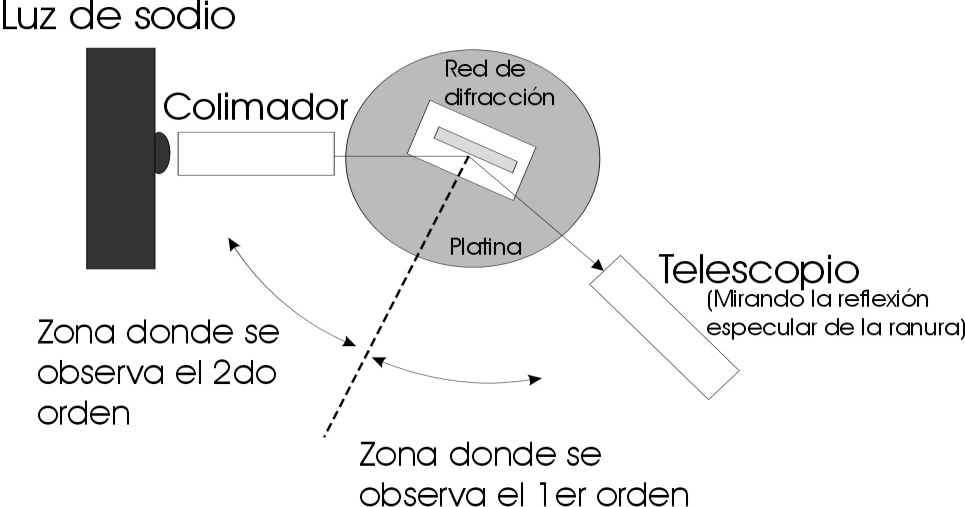
\includegraphics[width=8.5cm]{LG11--002.png}
    \caption{Esquema del dispositivo. Note la ubicación de la red respecto del haz proveniente de la lámpara de Na.
    }
    \label{fig:1}
\end{figure}

En la Figura \ref{fig:1} se muestra el dispositivo a montar. La red se coloca 
sobre la platina de modo que \'esta quede perpendicular al haz 
incidente y centrada, es decir que el haz debe incidir en forma 
paralela a la normal de la red ($\theta_0 = 0$). ?`Por qu\'e? Si 
as\'\i\ no fuera, ?`qu\'e precauci\'on debe tomar al realizar los 
c\'alculos?

        Para asegurarse incidencia normal se ubica el anteojo enfrentando al 
        colimador y se lee la posici\'on angular ($L_0$). A continuaci\'on, 
        se buscan los m\'aximos correspondientes al mayor orden de 
        interferencia visible; primero hacia un lado y luego hacia el otro,
        registrando los \'angulos correspondientes. Si la desviaci\'on respecto
        de $L_0$ correspondiente a un mismo orden de interferencia, es 
        id\'entica hacia ambos lados se puede considerar que la red est\'a 
        ubicada en forma perpendicular al haz incidente. (Justifique por qu\'e
        esta afirmaci\'on es v\'alida). Si observa que la red no est\'a 
        centrada, gire la platina levemente y determine nuevamente la 
        desviaci\'on de los m\'aximos hacia ambos lados hasta que sus 
        observaciones coincidan.

    \item {\bf Mediciones}. Conociendo la periodicidad de la red y midiendo los
        \'angulos asociados a los  m\'aximos de interferencia se pueden 
        calcular las longitudes de onda emitidas por la l\'ampara de sodio, a
        partir de la ecuaci\'on de la red. Mida todos los \'ordenes observables
        y construya un gr\'afico de $\sin \theta_m$ en funci\'on de $m$. 
        ?`Cu\'antas longitudes de onda espera observar?
        
        {\bf El doblete del sodio}. En la l\'ampara de sodio hay presentes,
        en realidad, dos longitudes 
        de onda correspondientes a lo que nuestros ojos perciben como un 
        color amarillo. Estas l\'\i neas de emisi\'on son muy cercanas y no es
        posible resolverlas en el primer orden de interferencia. 
        ?`A partir de qu\'e orden puede apreciar el doblete del sodio? 
        Intente medirlo.
\end{enumerate}

\section{Determinaci\'on de los l\'\i mites del espectro visible}

Reemplace ahora la l\'ampara de sodio por una de luz blanca y observe su  
espectro de emisi\'on empleando el mismo montaje experimental que utiliz\'o 
previamente. En estas condiciones, 

\begin{enumerate}
    \item Responda: el espectro observado, ?`es distinto del de la l\'ampara 
        de sodio? ?`En qu\'e aspectos? ?`A que se debe la diferencia? 
    \item Mida las longitudes de onda asociadas a los l\'\i mites que percibe.
\end{enumerate}


\section{Redes de difracci\'on por reflexi\'on}

Una red de reflexi\'on es una red de difracci\'on constituida por una serie
de surcos hechos sobre una superficie met\'alica. La mayor\'\i a de las redes
de reflexi\'on est\'an construidas de forma tal que la posici\'on del m\'aximo
de difracci\'on es diferente de la posici\'on del orden cero de interferencia.
De este modo se logra que la mayor intensidad de luz (asociada al 
m\'aximo principal de difracci\'on) est\'e dirigida hacia \'ordenes superiores
de interferencia donde la red tiene mayor poder resolvente. Este tipo de 
construcci\'on recibe el nombre de {\it blaze} o, en castellano, {\it
resplandor}. Con estas redes resulta conveniente trabajar en incidencia oblicua
(casi razante), a fin de poder observar mejor los distintos \'ordenes de
interferencia. 

No obstante sus diferencias con las redes de transmisi\'on, resulta f\'acil
mostrar que la ecuaci\'on para este tipo de redes es id\'entica a la obtenida
para aquellas. Mu\'estrelo. 

Dado que se trabaja con incidencia oblicua, es importante medir en forma 
precisa el \'angulo de incidencia. Para ello, emplearemos nuevamente el 
goni\'ometro. 

Una forma de fijar los \'angulos en el goni\'ometro en una posici\'on de 
referencia conocida consiste en colocar el \'angulo cero de la platina en 
forma coincidente con el haz incidente. Esto se logra observando la ranura
del colimador con el telescopio, ya que en esta posici\'on el colimador
y el telescopio forman un \'angulo de $\pi$~rad. Mueva entonces la platina
hasta hacer coincidir la marca de 180$^\circ$ con el cero del vernier del
telescopio. Coloque ahora la red poniendo atenci\'on a que quede centrada en
la platina, y de modo tal de lograr un \'angulo de incidencia no menor a 
65$^\circ$ (?`Por qu\'e?) Calcule, a partir de la medici\'on del \'angulo 
asociado al orden cero, la posici\'on de la normal de la red. Mida los 
\'angulos de cada orden y cada longitud de onda. A partir de los datos 
obtenidos, determine las longitudes de onda. 



% \section*{Ap\'endice}

<<<<<<< HEAD
=======



% \section*{Ap\'endice}

>>>>>>> ad104c7a42e80d40c124c0d895c6eb3e68874fce
% El goni\'ometro consta de una platina giratoria solidaria a un limbo graduado,
% sobre la cual se coloca la red. Un colimador, para crear un haz incidente de 
% rayos paralelos, y un anteojo que permite llevar el plano de observación al 
% infinito, el anteojo es móvil y posee un vernier para medir el ángulo de giro
% sobre el limbo graduado. El anteojo tiene un retículo en forma de cruz que 
% permite definir mejor las posiciones que se miden.

% Antes de medir, el dispositivo debe ser ajustado para trabajar bajo las 
% condiciones de difracción de Fraunhofer e incidencia normal. Para ello debe 
% enfocar el colimador y el anteojo. Primero se enfoca el anteojo mirando un 
% objeto distante (enfoque a infinito) desplazando el ocular del tubo. Luego se 
% enfoca el colimador enfrentándolo al anteojo y desplazando la rendija que se 
% halla adherida a él hasta obtener una imagen nítida de ella.

% A continuación se debe ubicar la red paralela al eje del goniómetro y 
% aproximadamente perpendicular al haz colimado. La red se encuentra paralela 
% al eje cuando la imagen de la rendija a través de la red se halle centrada 
% y paralela al eje vertical del retículo. Para lograr posicionarla 
% correctamente la platina cuenta con tres tornillos de nivelación.






        
%\begin{sabermas}
%Para saber mas haria falta leer un poco las siguientes referencias.
%indeed up to 90\% of the energy is in wave modes for the lower
%wavenumbers. While this results point that waves dominate the largescale
%dynamics, it is also clear that they do not govern the smaller scales.
%This puts theories in which eddies are not accounted for on.
%\end{sabermas}

\nocite{Alonso1998,Jenkins2001,Hecht1986}
\bibliographystyle{unsrt}
\bibliography{Bibliografia}

\end{document}
